\section{Computer Vision}
\label{sec:vision}
Various vision algorithms are needed for more careful perception and analysis of Pepper’s environment on object and human level. 
Usually, to start a certain task, our Pepper can detect and recognize different people, remember their names and some other features, and tracking them. 
Then, more skills will be shown for complex goals.  
For object-level environment reasoning, we build an object detection and recognition framework based on YOLO \cite{Redmon2018YOLOv3AI}, which is an interesting real-time algorithm. 
According to the competition scenario of RoboCup@Home, our object detection system can detect 50 classes of indoor objects in real time. 
To train our object detection network, we make a great dataset from OpenImages. 
We also match adjacent input frames to increase the robust of detection.

In some tasks we need a wide field of view, but the top 2D camera makes us disappointed. 
So we need to take some measures to expand Pepper’s original “eyes”. 
The method we choose is to stitch images from different perspectives, and a fusion algorithm follows to decrease the influence of illumination and geometric change. 
Now more visual candidates can be included for further processing.
\begin{figure}[h!]
\centering
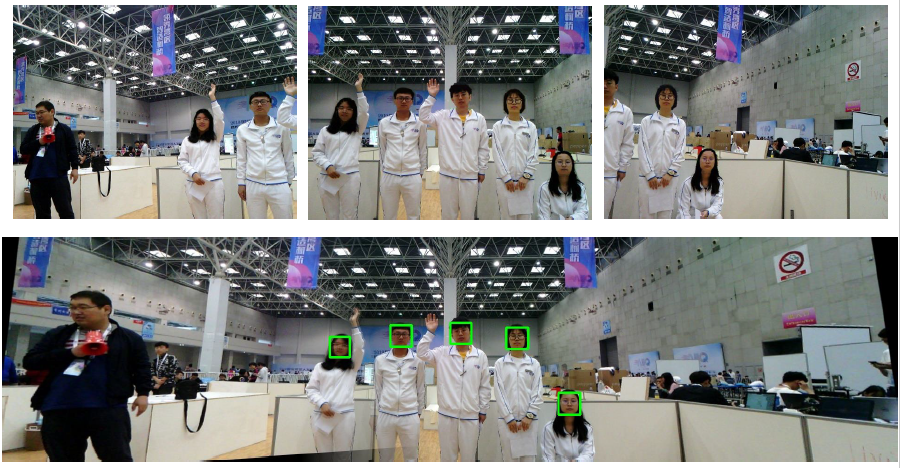
\includegraphics[width=1.\textwidth]{figs/vision1.png}
\caption{Image Stitch and Fusion to Detect in a Lager Field of View}
\label{fig:vision1}
\end{figure}

A more exciting visual module is human pose estimation. 
For this feature, we use OpenPose \cite{Cao_2017_CVPR} model to get a robust and real-time performance. 
With a non-parametric representation, we can detect associate body parts of multiple people in the input image stream. 
\begin{figure}[h!]
    \centering
    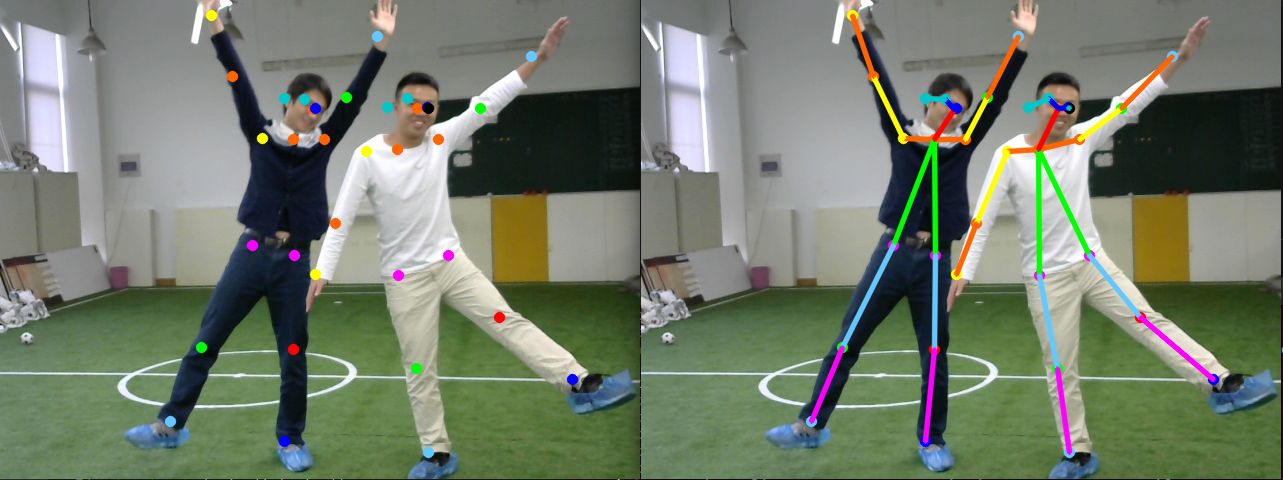
\includegraphics[width=1.\textwidth]{figs/vision2.png}
    \caption{Using OpenPose model to estimate body pose}
    \label{fig:vision2}
\end{figure}

The NAOqi system itself contains many interesting APIs, they may not have high precision, but are still useful for further development. 
For example, we can use some APIs to judge whether a person is standing or sitting, close or far away from the robot. 
These functions are also integrated to human-robot interaction modules.